\subsection{Filosofia Lean}
Il \textit{lean thinking} nasce come concettualizzazione di un sistema di management collaudato con risultati eccellenti: il \textit{Toyota Production System (TPS)}.

Le sue origini provengono dall’ambito manifatturiero ma oggi è applicato con successo a tutti i processi operativi: progettazione e sviluppo prodotto, logistica e amministrazione.

Tra il 1800 e 1910 il sistema di produzione era organizzato secondo le logiche tipiche dell’artigianato: caratterizzato da bassi volumi di produzione, elevata varietà di prodotti da unicità, scarsa divisione del lavoro e basso coordinamento, assenza di forme di automazione.

Tra il 1910 e il 1950 una nuova forma di capitalismo è emersa in seguito alla concentrazione del capitale industriale e finanziario in grandi imprese, per rispondere alla esigenza di ingenti investimenti in macchinari e impianti.

In queste grandi imprese industriali cominciò a diffondersi la produzione in serie e su larga scala nota come fordismo. Henry Ford\footnote{Dearborn, 30 luglio 1863 – Detroit, 7 aprile 1947 - Imprenditore statunitense, co-fondatore della Ford Motor Company} si ispirò alle teorie di Frederick Taylor\footnote{Germantown, 20 marzo 1856 – Filadelfia, 21 marzo 1915 - Ingegnere ed imprenditore statunitense, famoso per la sua ricerca sul miglioramento dell'efficienza dei metodi produttivi}, l’applicazione dei principi di \textit{“organizzazione scientifica del lavoro”}, di una divisione del lavoro molto spinta basata sull’analisi dei tempi e dei metodi e di un forte ricorso all’automazione, e introdusse per la produzione del modello \textit{Ford T} la catena di montaggio, ottenendo così una produzione di massa, altamente standardizzata, con una notevole diminuzione nei tempi di produzione. La produzione di massa è caratterizzata da una forte integrazione verticale e centralizzazione delle decisioni, un orientamento alla produzione di elevate quantità con alto livello di standardizzazione: l’attenzione non si focalizza sul flusso del materiale o prodotto quanto sulla produzione della maggior quantità possibile. Lo scollegamento dei processi produttivi fa sì che le scorte di semilavorati crescano notevolmente, la produzione non è programmata sulla base della domanda di mercato e i prodotti finiti vengono comunque spinti sulla rete di venditori (\textit{produzione push}).

Il modello sviluppato da \textit{Ford} fu da ispirazione per il sistema di produzione adottato da \textit{Toyota}\footnote{Casa automobilista giapponese} negli anni 40 che lo perfezionò per rispondere alle necessità di flessibilità della produzione e una disponibilità di infrastrutture minore.

Sotto la guida dell’ingegnere capo Taichii Ohono\footnote{Dalian, 29 febbraio 1912 – Toyota, 28 maggio 1990 - Ingegnere giapponese} \textit{Toyota} sviluppò il \textit{TPS} (\textit{Toyota Production System}), un sistema di produzione guidato dai principi di lotta agli sprechi e di miglioramento continuo, caratterizzato da una automazione limitata e flessibile, dalla polifunzionalità degli operatori e da una integrazione a rete.

Il termine \textit{“lean”} è divenuto popolare nel 1990 grazie al libro \textit{“La macchina che ha cambiato il mondo”} di \textit{Womack Jones} e \textit{Roos}. Essi hanno chiaramente illustrato per la prima volta, le notevoli differenze tra il sistema produttivo occidentale e il \textit{TPS}. Hanno definito gli elementi chiave che consentivano delle prestazioni superiori, come \textit{lean production} o produzione snella, snella perché il sistema produttivo giapponese ha permesso di utilizzare meno di tutto – meno sforzo umano, meno investimento di capitali, strutture, meno scorte e tempo – nella produzione, nello sviluppo del prodotto, nella fornitura e nella vendita.

\subsubsection{Concetti base della filosofia Lean}
Alla base del \textit{lean thinking} risiedono dei concetti fondamentali che rivoluzionano la cultura e il modo di operare all’interno dell’azienda:
\begin{itemize}
	\item \textbf{Attenzione al cliente.} La centralità del cliente è il punto di partenza e di arrivo di tutte le attività ed azioni messe in campo dall’azienda nel trasferire, attraverso i propri prodotti e servizi, il valore che il cliente si attende. Il cliente non è solo quello finale, il cliente “interno” è ugualmente importante. Il flusso di informazioni parte dal cliente fino ad arrivare alla ricerca e sviluppo: il dialogo con il cliente è fondamentale per identificare i fabbisogni e definire il valore.
	\item \textbf{Il contributo delle persone.} “Saper fare azienda”, o saper fare bene le cose (concetto giapponese \textit{Monozukuri}), è possibile solo partendo dalla capacità di gestire le persone (\textit{Hitozukuri}): lo sviluppo e il sostegno della competitività aziendale, con l’ottenimento di risultati significativi e duraturi, è possibile solamente con il continuo e costante allineamento del management e di tutte le persone che lavorano nell’azienda verso un obiettivo comune.
	\item \textbf{Lotta agli sprechi.} \textit{MUDA} è il termine giapponese che può essere tradotto come spreco. I \textit{MUDA} consistono in tutte le attività, che impegnano risorse ed energie, che non aggiungono valore al prodotto o al servizio e non danno quindi valore al cliente. Riconoscere gli sprechi è fondamentale per l’applicazione del \textit{lean thinking}.
	\item \textbf{Miglioramento continuo.} \textit{KAIZEN} in giapponese significa miglioramento continuo: nessun processo è perfetto ma può essere sempre migliorato. Tutto il personale dell’azienda, top management, dirigenti, responsabili, fino agli operatori, deve partecipare al processo di miglioramento condividendo obiettivi comuni e definiti.
\end{itemize}

\subsubsection{I 5 passi per la trasformazione Lean}
Nel libro \textit{“Lean Thinking” Womack} e \textit{Jones} hanno individuato i 5 principi chiave che devono essere accolti da una azienda per adottare il \textit{lean thinking}:
\begin{enumerate}
	\item \textbf{Value.} Ripensare al valore dal punto di vista del cliente. Solo una piccola parte delle azioni e del tempo totale che sono impiegate per produrre o fornire un servizio aggiungono effettivo valore per il cliente finale. Risulta quindi fondamentale definire chiaramente il valore di uno specifico prodotto o servizio dalla prospettiva del cliente, così che si possa procedere alla rimozione passo dopo passo di tutte le attività a non valore o \textit{MUDA}. Vengono anche definiti i 7 sprechi da evitare:
		\begin{enumerate}[label=\arabic*.]
			\item \textbf{Processi.} Presenza di operazioni inutili/inefficienti all’interno del ciclo di lavoro (tempi e metodi)
			\item \textbf{Sovrapproduzione.} Realizzare produzione non richiesta o anticipata o non necessaria in quel momento
			\item \textbf{Tempo.} Tempi di attesa dovuti a problemi di bilanciamento e/o mancata sincronizzazione tra le fasi del processo
			\item \textbf{Scorte.} Presenza di scorte eccessive di materiali/attrezzature lungo il processo
			\item \textbf{Movimenti.} Presenza di movimenti inutili e/o inefficienti e che quindi non aggiungono valore alla produzione
			\item \textbf{Difetti.} Presenza di difetti/ non conformità lungo il processo produttivo o segnalate dal cliente (interno/esterno)
			\item \textbf{Trasporto.} Presenza di inutili trasporti di materiali e attrezzature tra le varie fasi del processo, dovute a distanze/quantità
				non ottimizzate
		\end{enumerate}
		
		\textit{GEMBA} = luogo dove si crea il valore
	\item \textbf{Map.} Mappare il flusso del valore, i deve analizzare lo stato attuale e definire lo stato futuro per ciascuno dei 3 processi chiave aziendali:
		\begin{itemize}
			\item \textit{Product/Development:} definizione nuovi prodotti/servizio (dall’ideazione al benestare per la produzione)
			\item \textit{Order Fulfillment:} gestione ordini (dal ricevimento ordini alla consegna cliente)
			\item \textit{Production:} trasformazione fisica del prodotto (dalla MP\footnote{ Materia Prima} al PF\footnote{ Prodotto Finito})
		\end{itemize}
	\item \textbf{Flow.} Creare un flusso per ridurre il \textit{lead time}. La gestione del lavoro non viene fatta attraverso reparti successivi, i processi vengono riorganizzati in modo che il flusso di prodotti o attività scorrano senza interruzioni attraverso le varie fasi di aggiunta di valore, utilizzando l’insieme di strumenti e tecniche \textit{lean} per rimuovere tutti gli ostacoli dal flusso. La rimozione di tempo ed energie sprecate rappresenta una grande opportunità di miglioramento nell’efficienza qualitativa e quantitativa di una azienda, consentendo di focalizzare l’attenzione e gli sforzi alla creazione di valore
	\item \textbf{Pull.} Far tirare la produzione dal cliente: far sì che produzione e fornitura siano coordinate con le richieste di mercato
	\item \textbf{Perfection.} Miglioramento continuo. Creare un flusso e far tirare la produzione dal cliente comincia anche attraverso una radicale riorganizzazione dei processi ma i risultati divengono realmente significativi nel momento in cui tutti i passaggi sono collegati tra loro. Tecnica del \textit{PDCA}:
		\begin{itemize}
			\item \textbf{Plan}. Stabilire il \textit{target} del miglioramento
			\item \textbf{Do.} Implementare l’attività
			\item \textbf{Check.} Controllare il risultato
			\item \textbf{Act.} Standardizzare ciò che e stato fatto
		\end{itemize}
\end{enumerate}

\subsubsection{Le tecniche operative della filosofia Lean}
\paragraph{Value Stream Mapping}
La \textit{Value Stream Mapping}(\textit{VSM}) è lo strumento con cui si realizza la mappatura del flusso del valore di un prodotto o famiglia di prodotti; tale mappatura consente di evidenziare tutte le attività (a valore aggiunto o non a valore aggiunto) necessarie per la realizzazione del processo produttivo

\begin{figure}[H]
	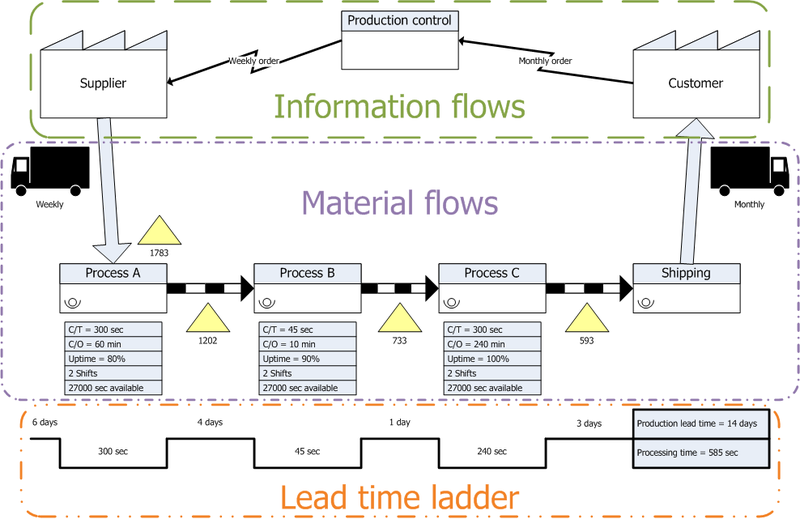
\includegraphics[width=0.7\linewidth]{resources/chapters/OrganizzazioneAziendale/images/vsm.png}
	\centering
	\caption{Esempio di \textit{VSM}}
\end{figure}

\paragraph{Spaghetti Chart}
Il diagramma “a spaghetti” consiste in una rappresentazione grafica degli spostamenti e percorsi compiuti da un prodotto lungo il flusso produttivo. Lo strumento mostra visivamente la linearità o la dispersione dei flussi. Può essere applicato anche per visualizzare gli spostamenti delle persone sul posto di lavoro

\begin{figure}[H]
	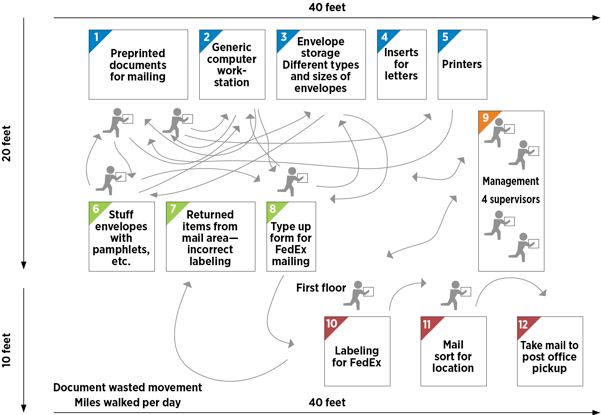
\includegraphics[width=0.8\linewidth]{resources/chapters/OrganizzazioneAziendale/images/spaghetti-chart.png}
	\centering
	\caption{Esempio di \textit{Spaghetti Chart}}
\end{figure}

\paragraph{Kanban}
La parola \textit{kanban} nasce in \textit{Toyota} e vuol dire “cartellino”, in quanto attraverso una gestione a vista di cartellini si evidenziava il consumo e quindi il fabbisogno di rifornimento di materiali alle fasi successive del processo

\begin{figure}[H]
	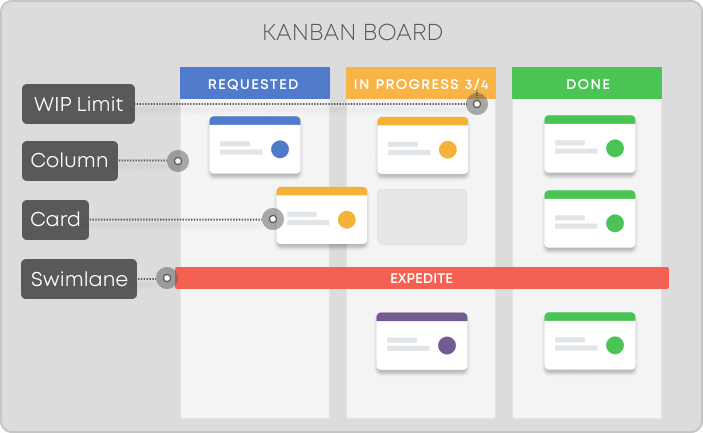
\includegraphics[width=0.8\linewidth]{resources/chapters/OrganizzazioneAziendale/images/kanban.png}
	\centering
	\caption{Esempio di \textit{Kanban}}
\end{figure}

\paragraph{Buffer FIFO}
I \textit{buffer FIFO} sono polmoni a capacità finita nei quali i prodotti avanzano in “fila indiana” garantendo che il primo prodotto che entra sia il primo ad uscire

\begin{figure}[H]
	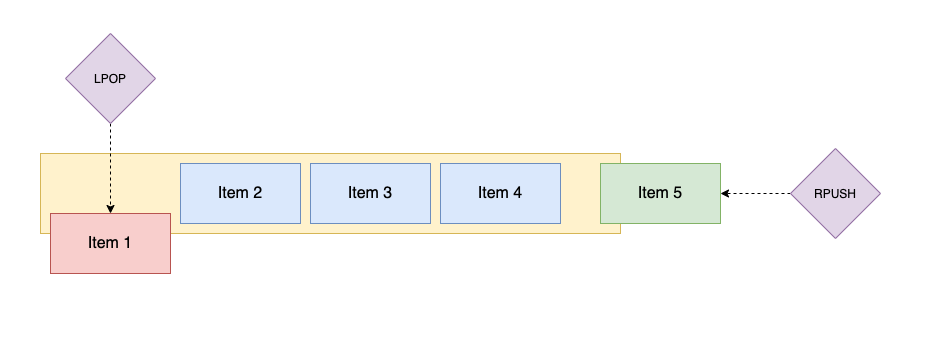
\includegraphics[width=0.8\linewidth]{resources/chapters/OrganizzazioneAziendale/images/fifo.png}
	\centering
	\caption{Esempio di \textit{Buffer Fifo}}
\end{figure}

\paragraph{Total Productive Management}
L’obiettivo del \textit{TPM} (\textit{Total Productive Management}) è quello di ridurre i guasti e le relative attività di manutenzione in emergenza, a favore di manutenzione preventiva (ciclica o su condizione). Il \textit{TPM} richiede inoltre una importante collaborazione del personale di produzione nelle attività di manutenzione autonoma (pulizia, ispezione, ecc...)

\paragraph{Le 5 "S"}
La tecnica \textit{“Five S”} è stata sviluppata in \textit{Toyota} al fine di fornire una guida operativa per l’organizzazione del posto di lavoro, la gestione a vista ed il mantenimento sul posto di lavoro degli standard di ordine e pulizia. Il motto per le \textit{5S} è un posto per ogni cosa ed ogni cosa al suo posto.

L’approccio 5S comporta la realizzazione dei seguenti 5 passi:
\begin{enumerate}
	\item \textbf{Seiri (separare):} separare le cose utili dalle inutili
	\item \textbf{Seiton (sistemare):} identificare e definire l’allocazione delle cose necessarie sul posto di lavoro (materiali, attrezzature, documenti)
	\item \textbf{Seiri (spolverare/pulire):} effettuare una pulizia intelligente del posto di lavoro
	\item \textbf{Seiketsu (standardizzare):} definire gli standard operativi per mantenere ordine e pulizia sul posto di lavoro
	\item \textbf{Shitsuke (seguire le regole):} diffondere gli standard operativi di ordine e pulizia e verificarne il rispetto da parte del personale
\end{enumerate}

\paragraph{Visula Management Systems}
Insieme di tecniche e strumenti per migliorare la gestione a vista sul posto di lavoro (cartellonistica, bacheche, righe a terra, sistemi di controllo stati macchina, sistemi di identificazione materiali/attrezzature, ecc...)


\paragraph{Poka Yoke}
Con il termine \textit{poka yoke} in \textit{Toyota} si identificavano sistemi o procedure che impediscono l’avanzamento nel processo di prodotti difettosi, intercettando gli errori (soprattutto umani) che stanno alla base dei difetti stessi.

Tali sistemi si chiamano anche \textit{“mistake proof”} (a prova d’errore) o \textit{“fool proof”} (a prova di scemo)


